\documentclass[12pt]{article}
\usepackage[english]{babel}
\usepackage{natbib}
\usepackage{url}
\usepackage[utf8x]{inputenc}
\usepackage{amsmath}
\usepackage{graphicx}
\graphicspath{{images/}}
\usepackage{parskip}
\usepackage{fancyhdr}
\usepackage{vmargin}
\setmarginsrb{3 cm}{2.5 cm}{3 cm}{2.5 cm}{1 cm}{1.5 cm}{1 cm}{1.5 cm}
\usepackage{booktabs}
\usepackage[pdftex]{hyperref}
\usepackage{hyperref}
\usepackage{graphicx}
\usepackage{epstopdf}
\usepackage{booktabs} 

\usepackage{listings}
\usepackage{color} %red, green, blue, yellow, cyan, magenta, black, white
\definecolor{mygreen}{RGB}{28,172,0} % color values Red, Green, Blue
\definecolor{mylilas}{RGB}{170,55,241}




\title{Report for Programming Exercise}								% Title
\author{Murat Kumru}								% Author
\date{29.11.2017}											% Date

\makeatletter
\let\thetitle\@title
\let\theauthor\@author
\let\thedate\@date
\makeatother

\pagestyle{fancy}
\fancyhf{}
\rhead{\theauthor}
\lhead{\thetitle}
\cfoot{\thepage}

\begin{document}

%%%%%%%%%%%%%%%%%%%%%%%%%%%%%%%%%%%%%%%%%%%%%%%%%%%%%%%%%%%%%%%%%%%%%%%%%%%%%%%%%%%%%%%%%

\begin{titlepage}
	\centering
    \vspace*{0.5 cm}
    
\includegraphics[scale = 0.3]{odtuLogo.png}\\[1.0 cm]	% University Logo
    \textsc{\LARGE Middle East Technical University}\\[2.0 cm]	% University Name
	\textsc{\Large EE 586}\\[0.5 cm]				% Course Code
	\textsc{\large Artificial Intelligence}\\[0.5 cm]				% Course Name
	\rule{\linewidth}{0.2 mm} \\[0.4 cm]
	{ \huge \bfseries \thetitle}\\
	\rule{\linewidth}{0.2 mm} \\[1.5 cm]
	
	\begin{minipage}{0.4\textwidth}
		\begin{flushleft} \large
			\emph{Author:}\\
			\theauthor
			\end{flushleft}
			\end{minipage}~
			\begin{minipage}{0.4\textwidth}
			\begin{flushright} \large
			\emph{Student Number:} \\
			1626449									% Your Student Number
		\end{flushright}
	\end{minipage}\\[2 cm]
	
	{\large \thedate}\\[2 cm]
 
	\vfill
	
\end{titlepage}

%%%%%%%%%%%%%%%%%%%%%%%%%%%%%%%%%%%%%%%%%%%%%%%%%%%%%%%%%%%%%%%%%%%%%%%%%%%%%%%%%%%%%%%%%

%\tableofcontents
%\pagebreak

%%%%%%%%%%%%%%%%%%%%%%%%%%%%%%%%%%%%%%%%%%%%%%%%%%%%%%%%%%%%%%%%%%%%%%%%%%%%%%%%%%%%%%%%%

%\section{Introduction}
%An open-source template Latex format of this report is obtained from \cite{ReportTemplate}.


\section{Answers}
\begin{enumerate}
	\item [\textbf{1}] 
	First of all, the whole program is written in Matlab environment. 
	All related information used to describe a puzzle configuration is stored in a data structure called \textit{Node}. 
	Considering remarkable computational advantages in manipulation of matrices and vectors by Matlab, \textit{Nodes} are implemented to be just column vectors with specified order of elements. 
	To illustrate, first \textit{n entities} of a \textit{Node} vector correspond to the numbers on the tiles stored in an ordered fashion. 
	This portion of a \textit{Node} is called \textit{State}. 
	In state vector, 0 (zero) is used as a placeholder for the free spot in the puzzle.	
	The rest of the vector comprises of a \textit{nodeID} (which is unique to each node), \textit{parentID} (serving as a back pointer) and \textit{cost} (to reach that node) as illustrated in Fig. \ref{fig:NodeStruct}. 
	Note that, if A* search algorithm is to be employed, than \textit{Node} vector is appended by a heuristic value and a scalar obtained by adding the heuristic and the cost. 
		
	\begin{figure}[!htb]
		\centering
		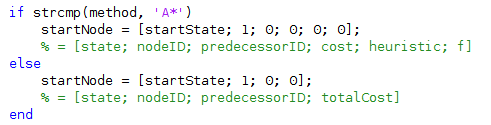
\includegraphics[width=.7\textwidth]{images/NodeDefinition.png}
		\caption{An example code snippet initializing a Node called \textit{startNode}}
		\centering
		\label{fig:NodeStruct}
	\end{figure}
	
	Furthermore, \textit{"previously visited"} and  \textit{"to be explored"} Nodes are also stored in matrices by simply concatenating related \textit{Nodes}.
	
	
	\item [\textbf{2}] To launch Graphical User Interface (GUI),  $user\_interface.m$ in the project directory is to be opened and run in Matlab environment. 
	Fig. \ref{fig:UI1} and Fig. \ref{fig:UI2} depict snapshots taken during different simulations.
	Via the GUI, a user can
		\begin{itemize}
			\item select the search algorithm to be used,
			\item track instantaneous state of the puzzle through free-run simulations,
			\item set any desired goal state,
			\item set an initial state or choose to assign a random one,
			\item start/stop/pause a free-run simulation,
			\item carry out single step iterations (Note that, in this mode, the solution is not obtained before presenting the result to the user. On the contrary, while the algorithm attempts to solve the problem, it simultaneously informs the user about configuration.)
			\item perform Monte Carlo simulations with desired properties.
		\end{itemize}

	\begin{figure}[!htb]
		\centering
		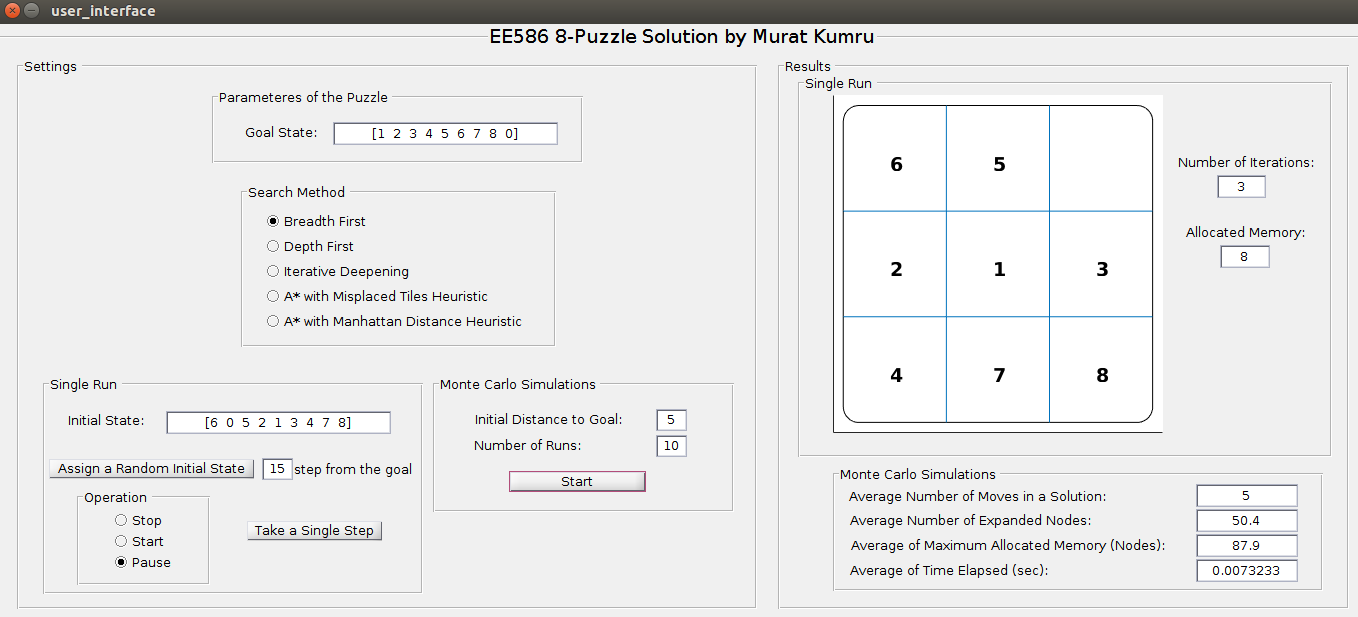
\includegraphics[width=1\textwidth]{images/UI_snapshot1.png}
		\caption{A view from GUI when the puzzle to be solved is 3-by-3}
		\centering
		\label{fig:UI1}
	\end{figure}

		\begin{figure}[!htb]
		\centering
		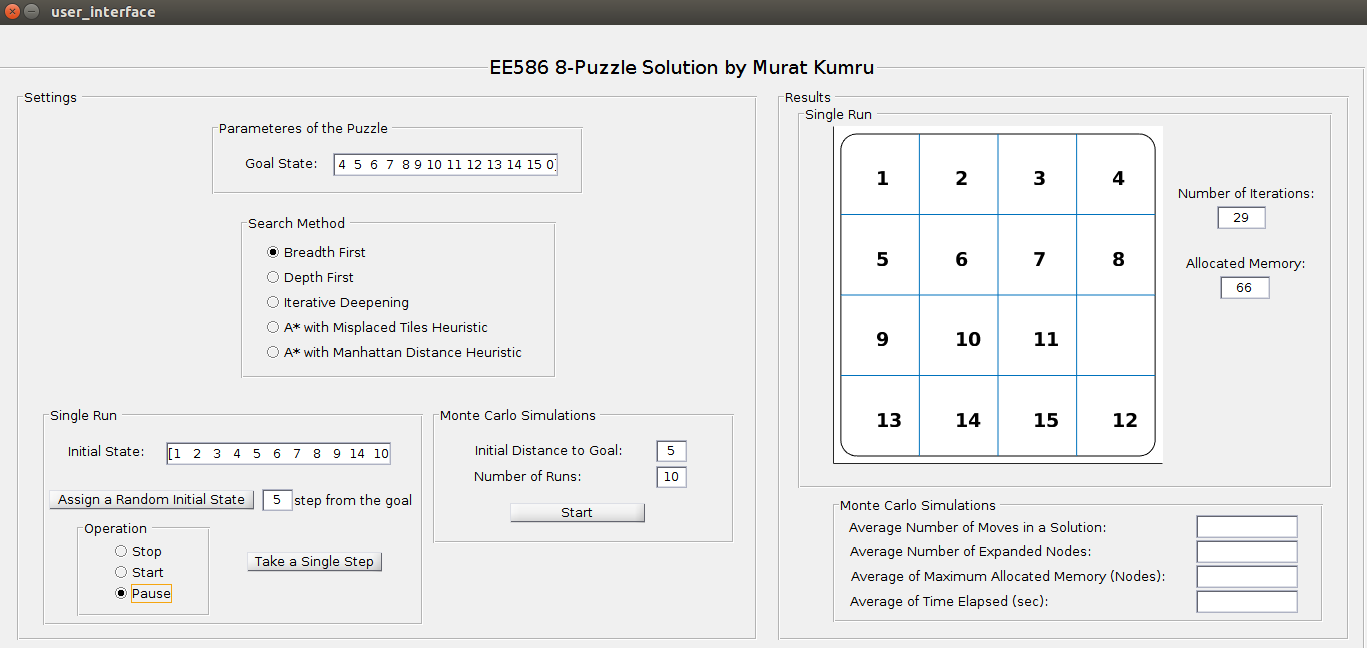
\includegraphics[width=1\textwidth]{images/UI_snapshot2.png}
		\caption{A view from GUI when the puzzle to be solved is 4-by-4}
		\centering
		\label{fig:UI2}
	\end{figure}	
	
	\item [\textbf{3}] The function named as \textit{successors()} can be found in the project directory. It has the ability to handle \textit{L-puzzle} case. A snapshot of the implementation is included in the Appendix section.
	
	\item [\textbf{4}] For the initial state given in Fig. \ref{fig:InitState}, the program is run with \textit{Breadth First Search(BFS)} algorithm.
		
	\begin{figure}[!htb]
		\centering
		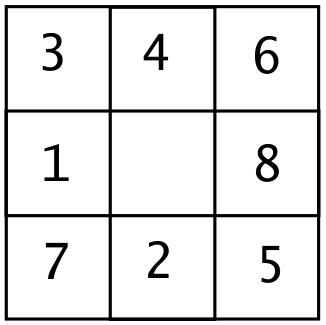
\includegraphics[width=.25\textwidth]{images/InitialState.png}
		\caption{Initial state of the puzzle}
		\centering
		\label{fig:InitState}
	\end{figure}
	
	\begin{enumerate}
		\item 2230 distinct \textit{Nodes} have been visited to find the optimum sequence of the puzzle.
		\item There are 12 tile moves in the optimum sequence.
		\item It takes about 0.85 seconds for the algorithm to end up with the solution.		
	\end{enumerate}

	\item [\textbf{5}] In this step, \textit{Depth First Search (DFS)} is considered.
	
	Depth First Search is implemented with an addition of a simple trick. 
	Stemmed from the nature of this puzzle problem, it is possible to run into the same nodes in separate branches of search. 
	This "problem" is tackled by not discarding a previously visited successor immediately, instead it is modified to compare the current version of the successor the previous one in terms of their costs. 
	However, the implementation do not end up with satisfying results. It took about 1.5 hour for the program to throw an out of memory error when the number of the explored nodes is around 90000.
	On the other hand, the procedure followed by the algorithm is verified to be consistent with the expectations coming from theoretical analysis of the algorithm.
	
	\item [\textbf{6}] In this step, \textit{Iterative Deepening Search (IDS)} is considered.
	IDS is built by giving the DFS an incremental control mechanism of maximum allowed depth. 
	The resultant observations are as follows:
	
	\begin{enumerate}
		\item 2074 distinct \textit{Nodes} have been visited to find the optimum sequence of the puzzle.
		\item There are 12 tile moves in the optimum sequence.
		\item It takes about 2.5 seconds for the algorithm to end up with the solution.		
	\end{enumerate}

	\item [\textbf{7}]
	\begin{enumerate}
		\item 	Making use of additional information provided by a heuristic function about \textit{Nodes} position with regard to the goal, \textit{A*} is expected to present computational advantage over aforementioned algorithms. 
		It essentially makes \textit{educated} guesses while selecting the next \textit{Nodes} to be explored. 
		Therefore, the more informative or explicit the heuristic function gets, the better performance is to be captured.
		With this in mind, Manhattan Distance serves a more comprehensive analysis of the problem.
		\item \textit{heuristic\_misplaced} and \textit{heuristic\_manhattan} functions are included in the directory.
		\item For two heuristic functions, following results are obtained:
		\begin{table}[h]
			\centering
			\caption{Comparison of two heuristic functions}
			\label{table: A* Comparison}
			\begin{tabular}{@{}ccc@{}}
				\toprule
				& Heuristic: Misplaced & Heuristic: Manhattan \\ \midrule
				\# of Moves          & 12                   & 12                   \\
				\# of Explored Nodes & 113                  & 24                   \\
				Elapsed Time (msec)  & 80.3                 & 61.7                 \\ \bottomrule
			\end{tabular}
		\end{table}
		
		\end{enumerate}
	
	\item [\textbf{8}]
	\begin{enumerate}
		\item [(a)] Desired number of random states at distance \textit{d} steps from the goal state are produced by \textit{produce\_random\_puzzle.m} function. A snapshot of the function is included in Appendix section.
		\item [(b)-(g)] For each search algorithm, Monte Carlo simulations with parameters \newline$ N=20,\ True\ Distance = \{1,\ 3,\ 5,\ 10,\ 15\}$ are conducted. 
		Note that due to the inconvenience in the operation of \textit{Depth First Search}, it is excluded from simulations and comparisons.
		
		Results are presented by Fig. \ref{fig:MCmove}- \ref{fig:MCtime}. 
		In the figures, data marks indicate the points at which MC simulations are performed, interpolating lines are just added to be able to interpret the findings.
		
		In Fig. \ref{fig:MCmove}, it is seen that all of the algorithms are able to find the sequence with minimum number of tile moves. 
		Moreover, in some cases, the averaged number of moves are observed to be less than the corresponding true distance which brings questions into mind.
		This results from the production process of random initial  states. 
		Although we produce random samples by moving tiles in an iterative fashion and preventing any possible loops, it does not guarantee not to have any path reaching to the goal with less number of tile moves.
		
		In Fig. \ref{fig:MCvisited}-\ref{fig:MCtime}, with increasing distance between the goal and initial states, the number of stored \textit{Nodes} and time spent to process these nodes increase for all algorithms as expected. 
		With respect to the dominance of exponential characteristic in the allocated memory and number of visited \textit{Nodes}, the algorithms are listed as BFS, IDS, A* with Misplaced Heuristic and A* with Manhattan Heuristic in a descending order.
		A* is detected to be the best performing algorithm for all cases.
		
	\end{enumerate}


	\begin{figure}[htb]
		\centering
		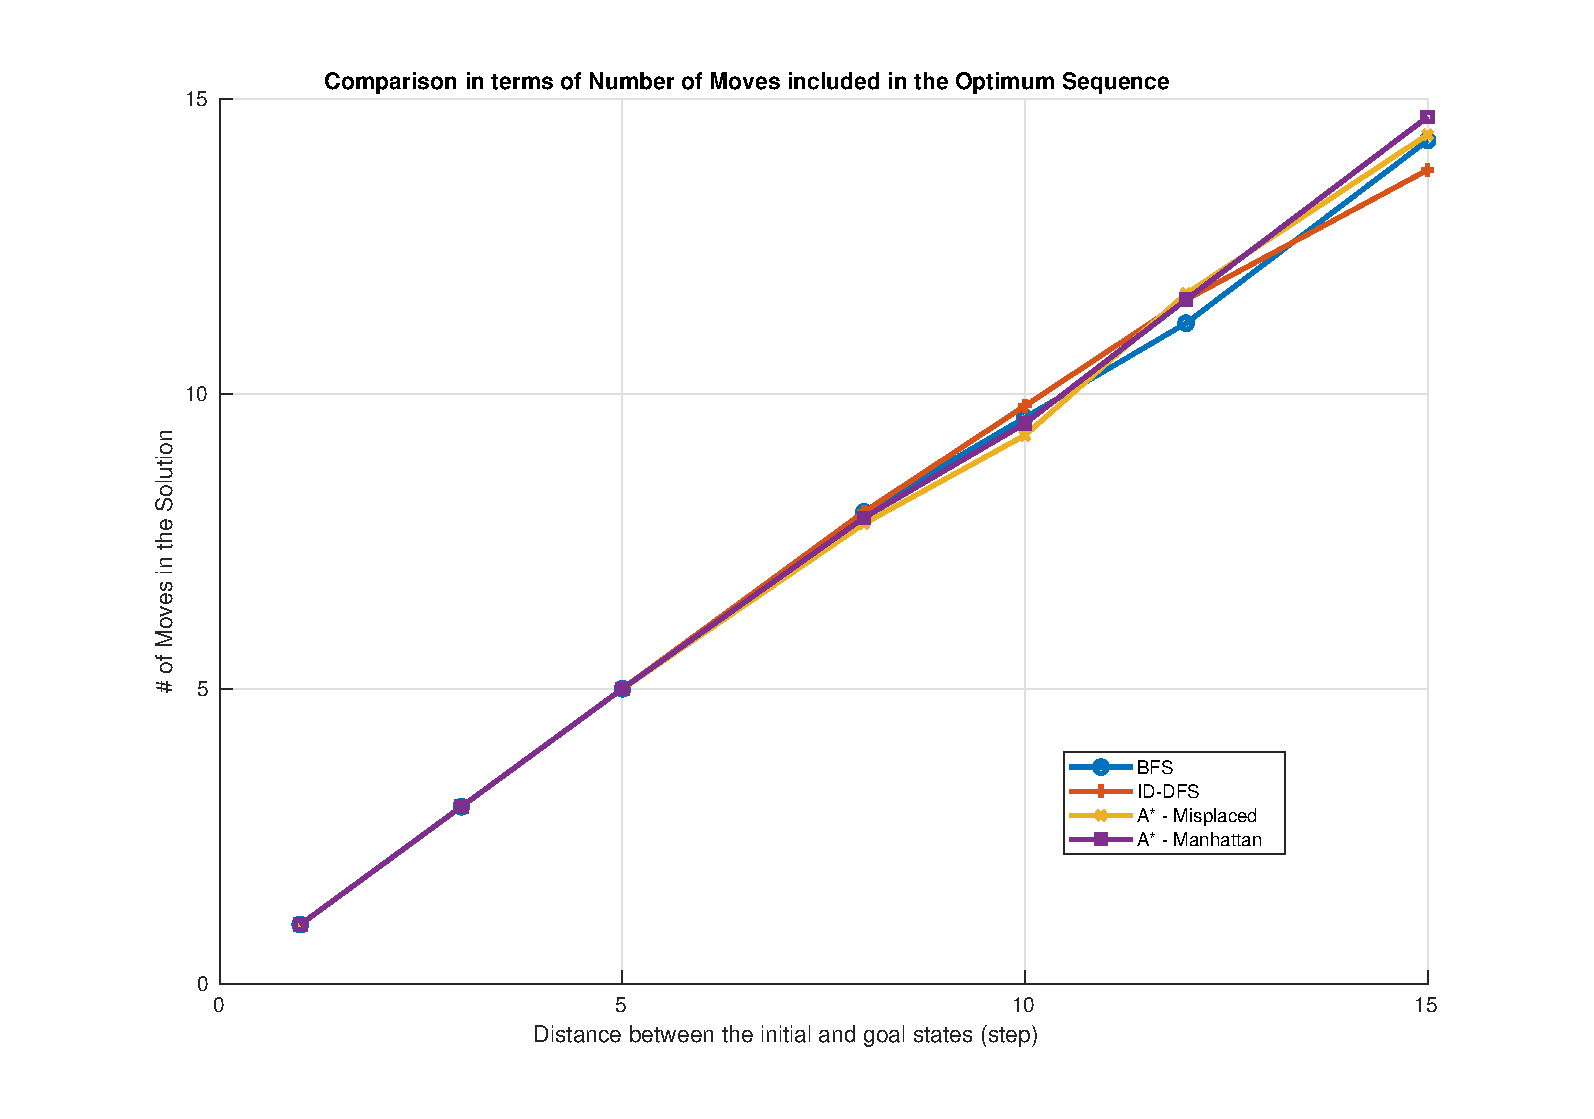
\includegraphics[width=1\columnwidth]{images/Q8_numMoves.eps}
		\caption{Comparison w.r.t. average number of moves in solutions}
		\label{fig:MCmove}
	\end{figure}

	\begin{figure}[htb]
		\centering
		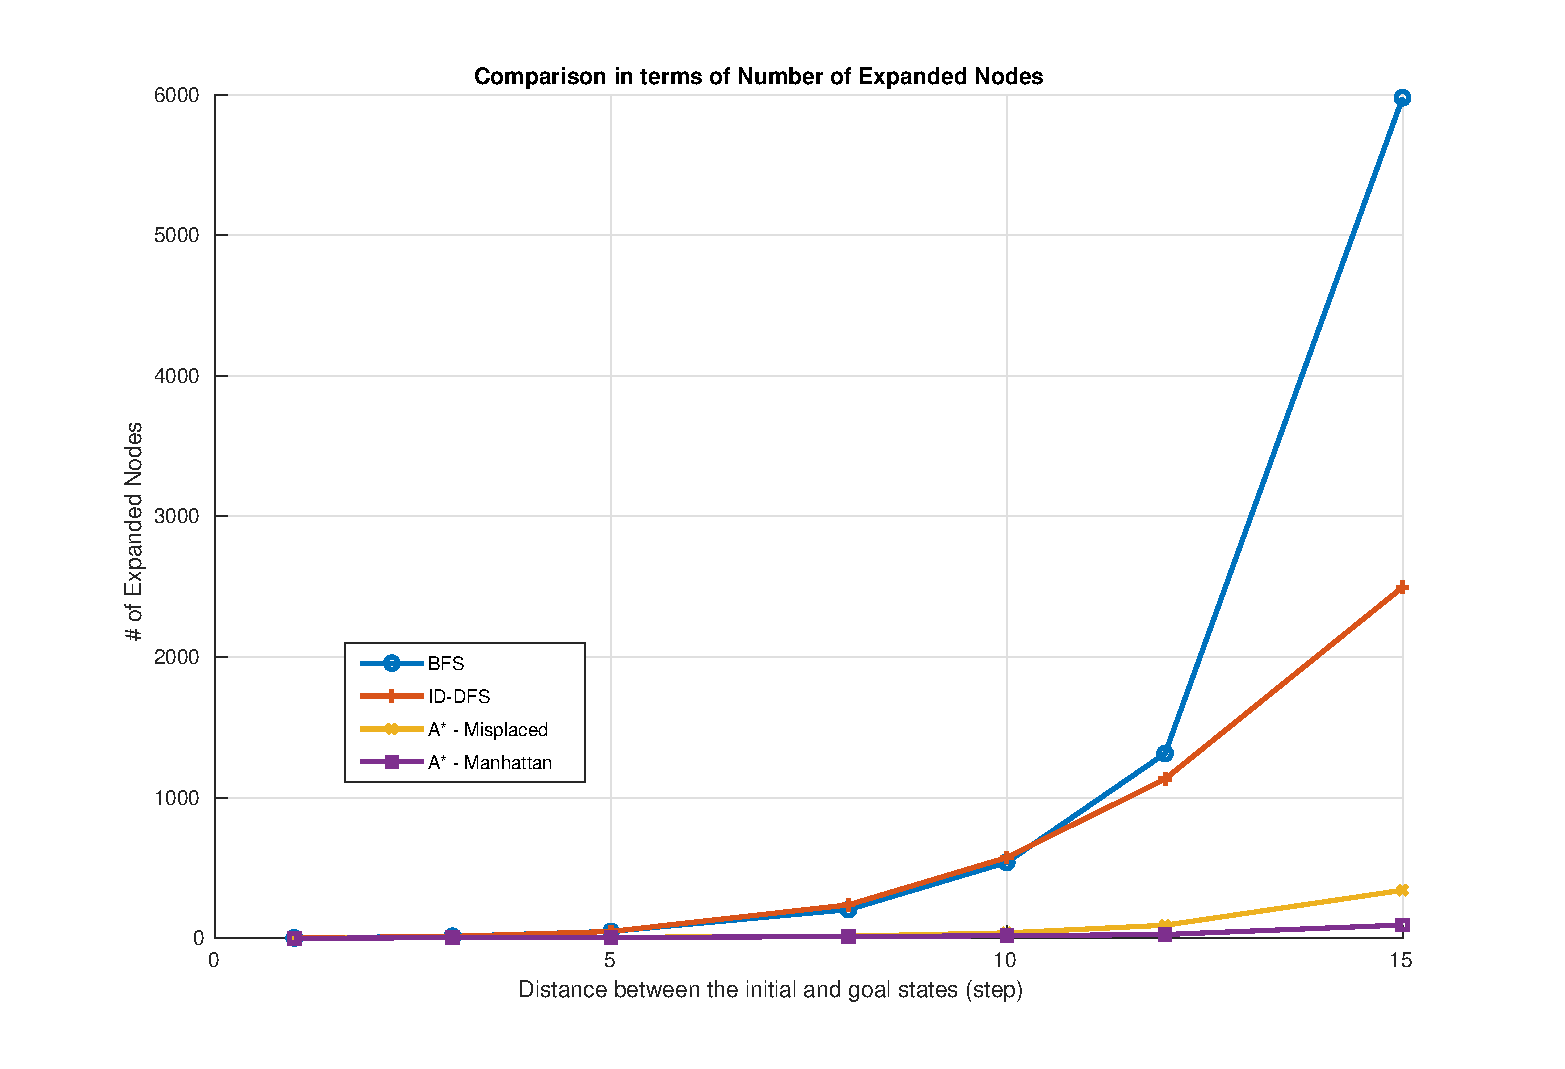
\includegraphics[width=.9\columnwidth]{images/Q8_numVisitedNodes.eps}
		\caption{Comparison w.r.t. average number of visited node throughout process}
		\label{fig:MCvisited}
	\end{figure}

	\begin{figure}[htb]
		\centering
		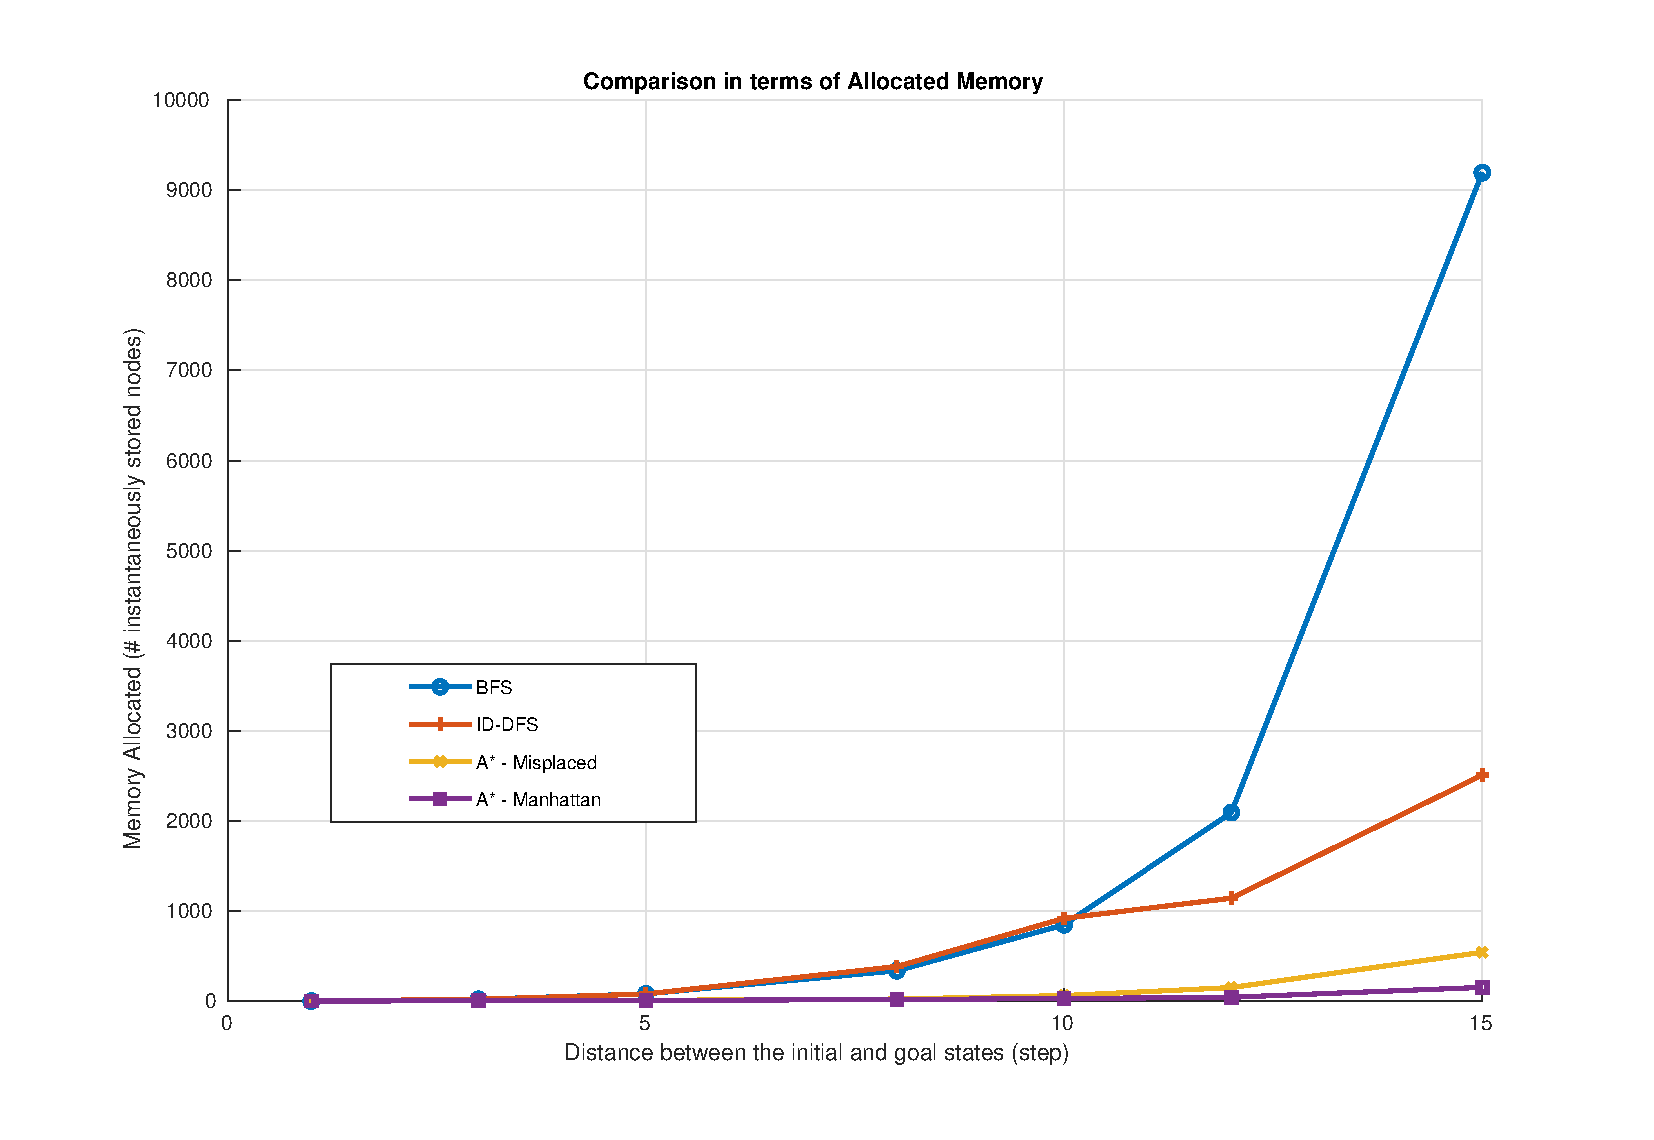
\includegraphics[width=.9\columnwidth]{images/Q8_allocatedMemory.eps}
		\caption{Comparison w.r.t. average allocated memory in terms of \textit{Nodes}}
		\label{fig:MCallocated}
	\end{figure}

	\begin{figure}[htb]
		\centering
		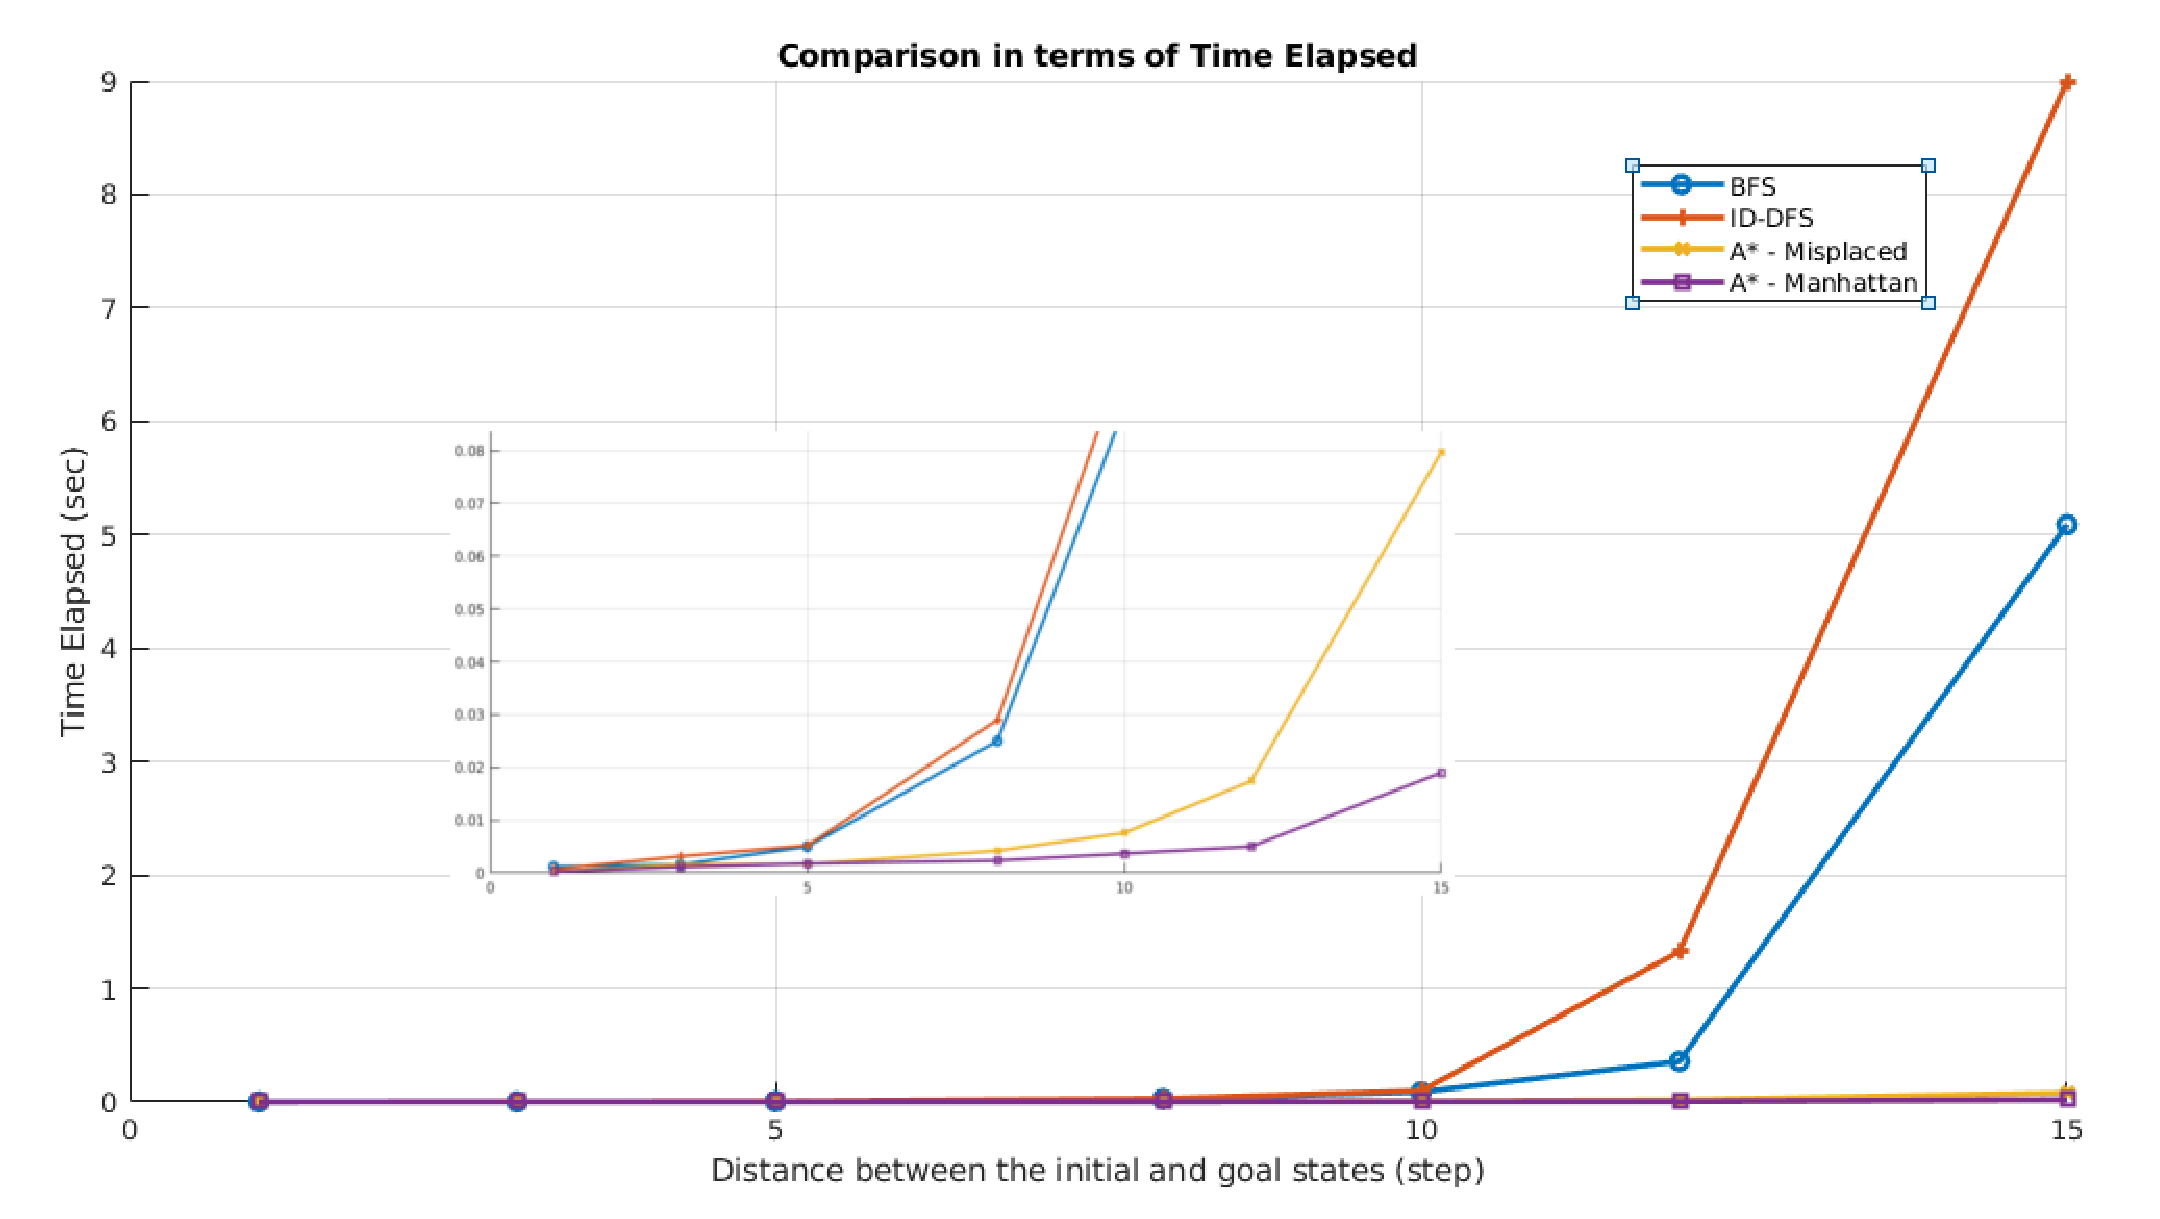
\includegraphics[width=.8\columnwidth]{images/Q8_timeElapsed.eps}
		\caption{Comparison w.r.t. time spent for simulations}
		\label{fig:MCtime}
	\end{figure}			 
			
			
	\item [\textbf{9}]
	In this step, A* Search algorithm with Manhattan Distance heuristic is scrutinized for puzzles with various dimensions. 
	For each size, random initial states are generated to be 15 steps away from the goal. 
	Number of Monte Carlo simulations are 20 for all scenarios.
	Puzzle sizes of 3-by-3, 5-by-5, 8-by-8, 10-by-10, 12-by-12, 15-by-15, 20-by-20, 25-by-25, and 30-by-30 cases are examined.
	Corresponding results are revealed by Fig. \ref{fig:Q9}.
	It is observed that the number of visited and queued \textit{Nodes} does not depend on the size of the puzzle. 
	On the other hand, the amount of utilized storage increases by increasing puzzle dimension since storing a \textit{Node} of a rather large puzzle takes more memory compared to the smaller ones.
	
	\begin{figure}[htb]
		\centering
		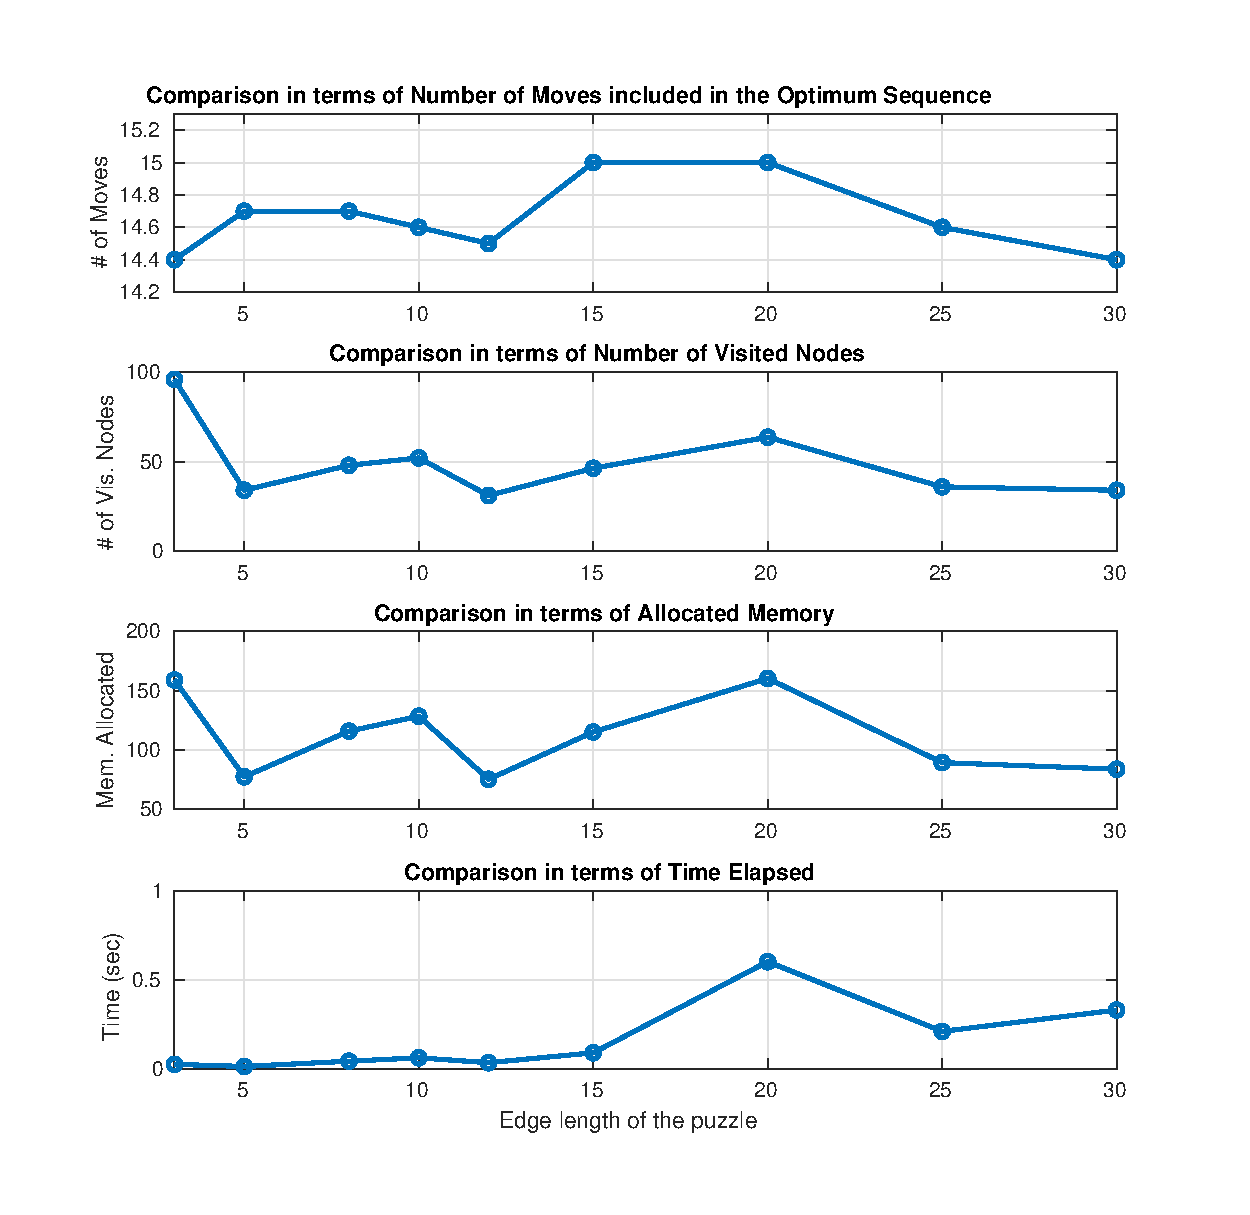
\includegraphics[width=0.8\columnwidth]{images/Q9.eps}
		\caption{Performance analysis of A* for various puzzle dimensions}
		\label{fig:Q9}
	\end{figure}

\end{enumerate}

\appendix
 
\begin{figure}[htb]
	\centering
	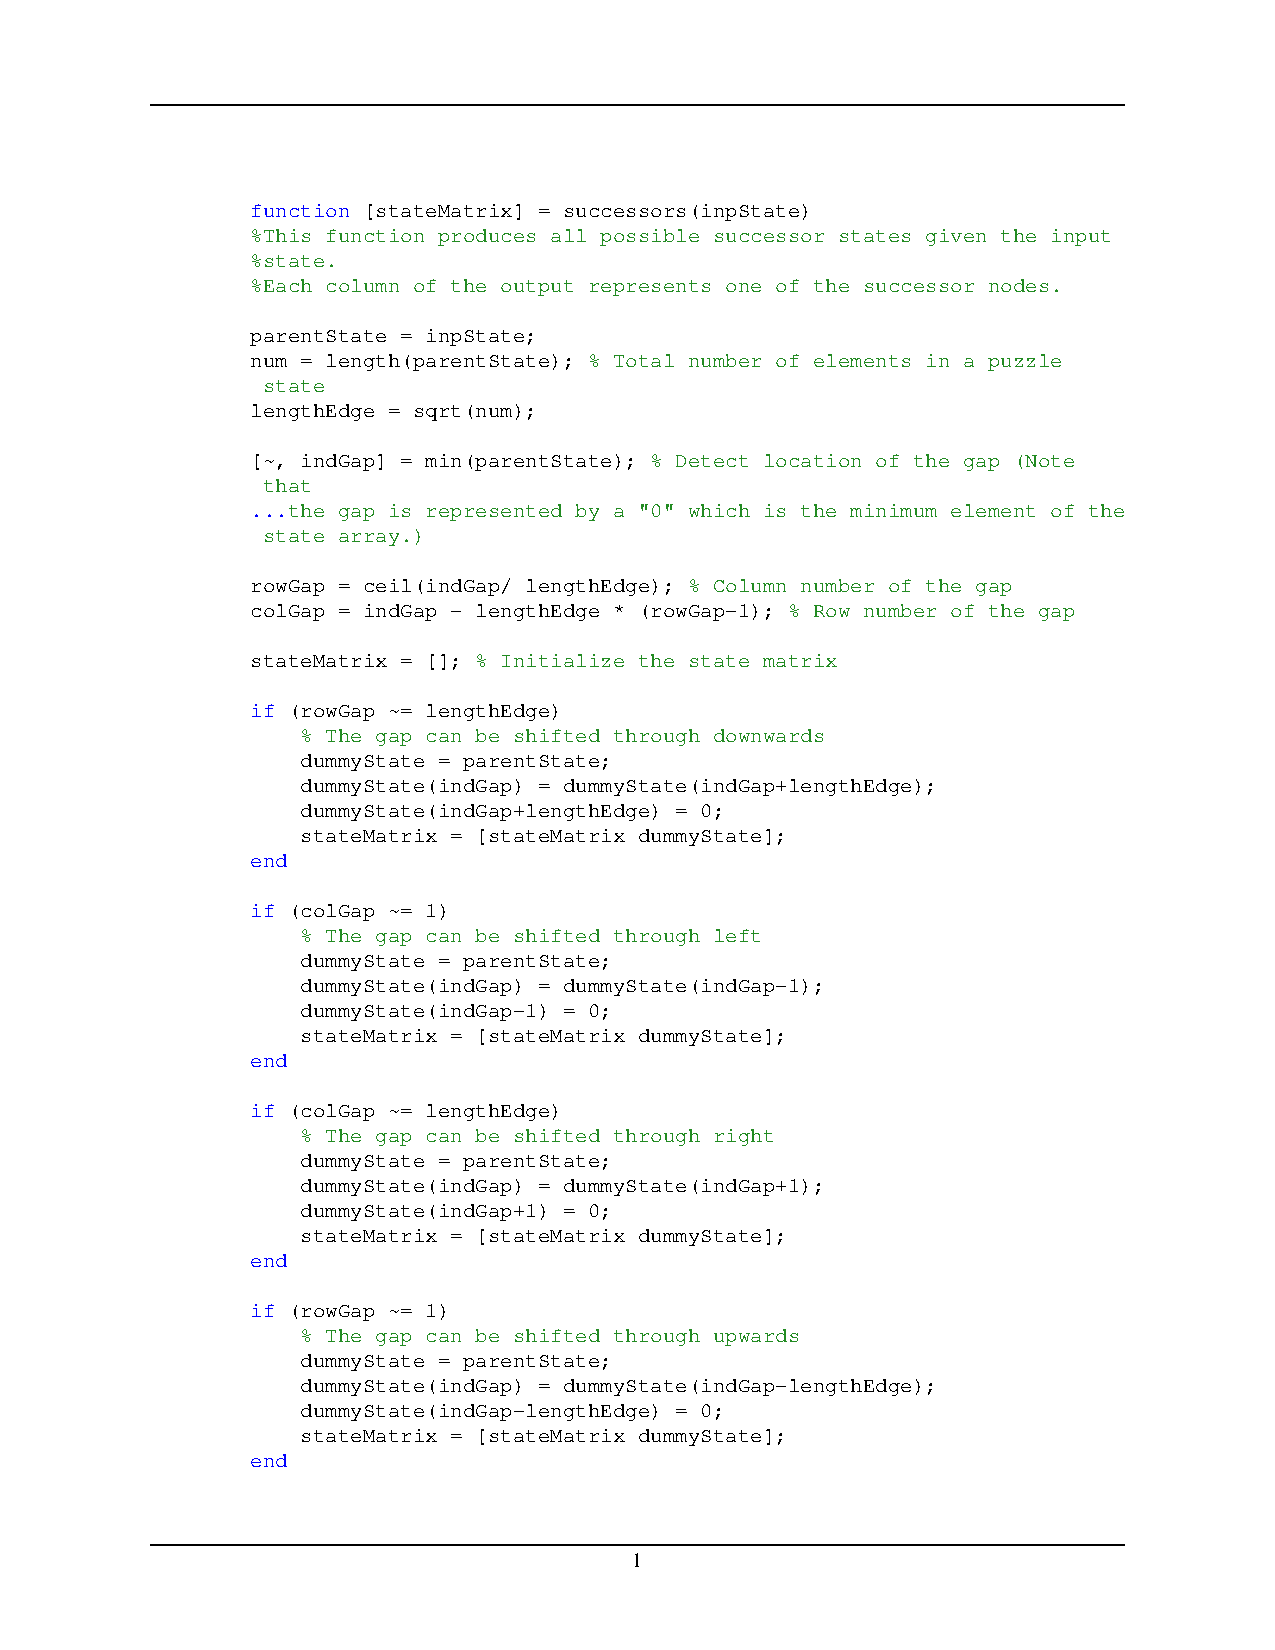
\includegraphics[width=1\columnwidth]{images/Code_successors.pdf}
	\caption{Implementation: \textit{successors} function}
	\label{}
\end{figure}

\begin{figure}[htb]
	\centering
	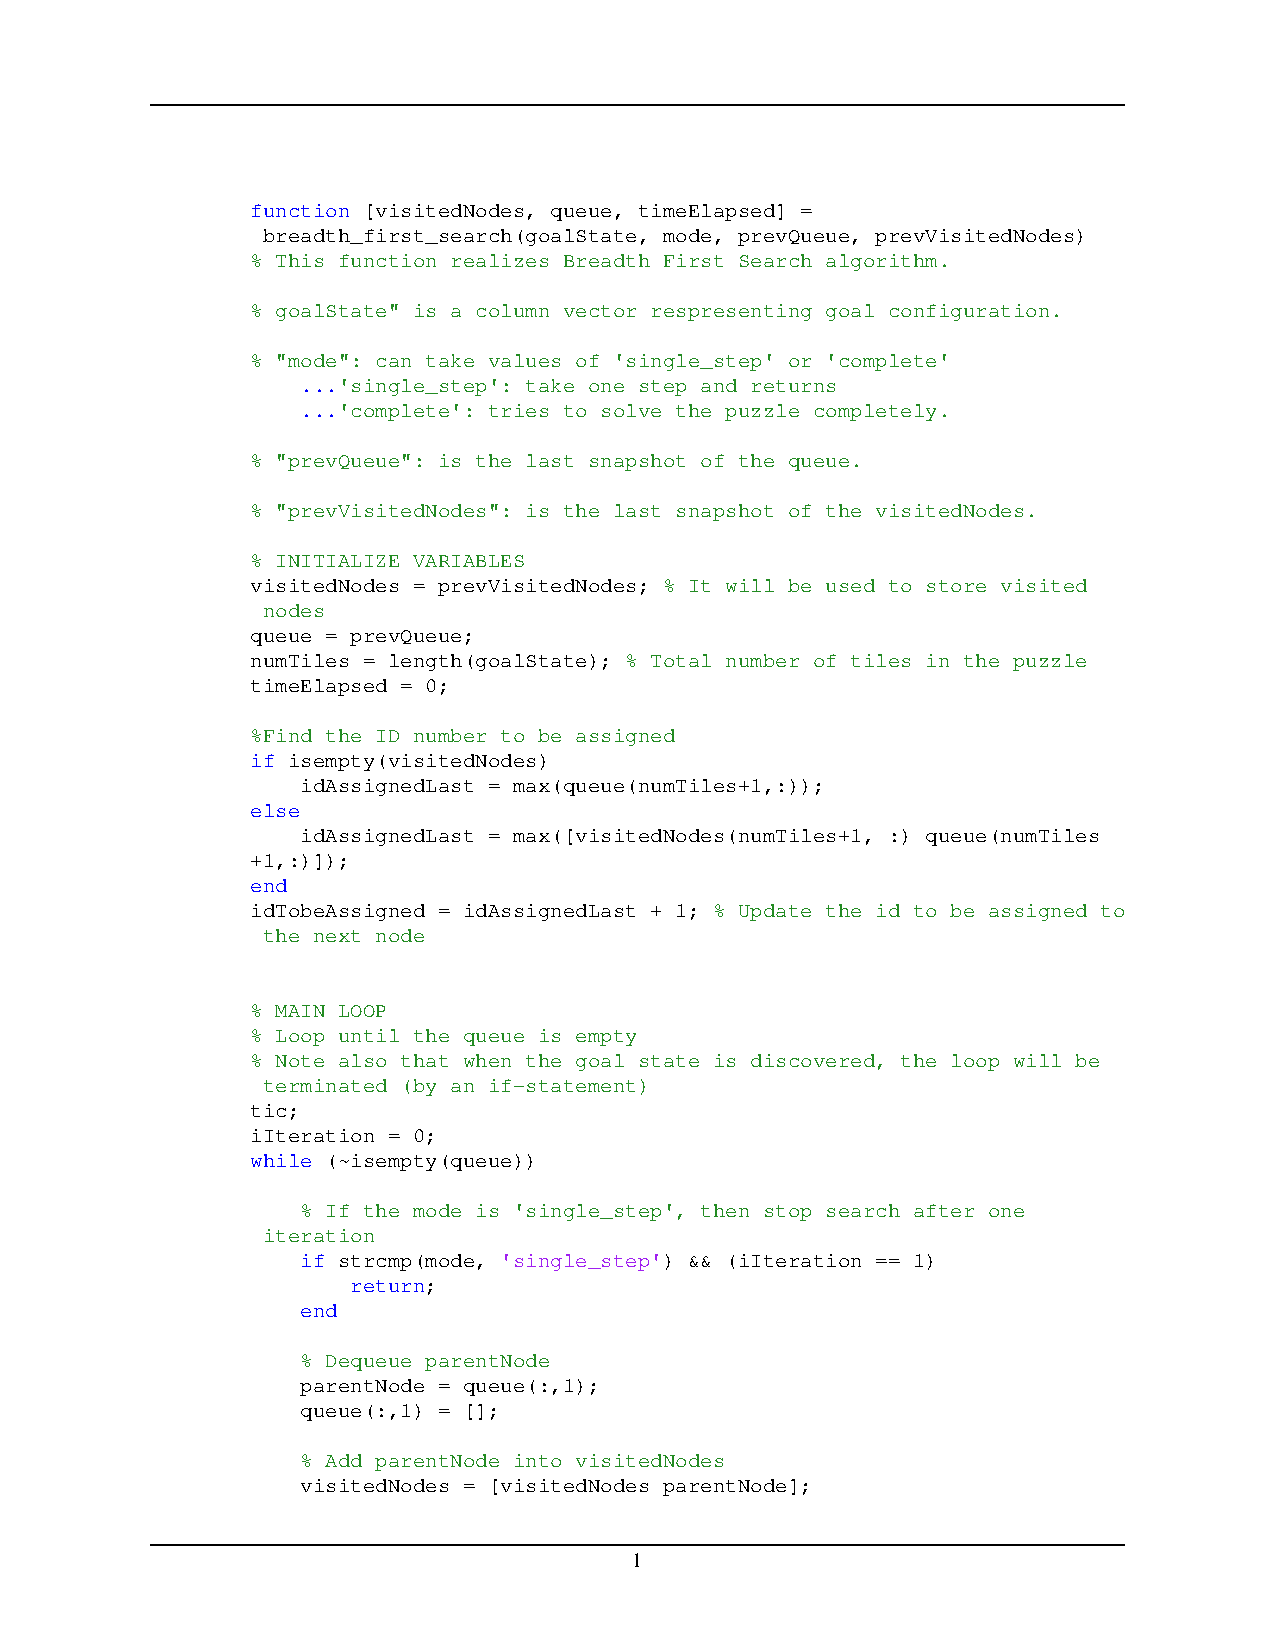
\includegraphics[width=1\columnwidth]{images/Code_breadth_first_search.pdf}
	\caption{Implementation: \textit{breadth\_first\_search} function}
	\label{}
\end{figure}

\begin{figure}[htb]
	\centering
	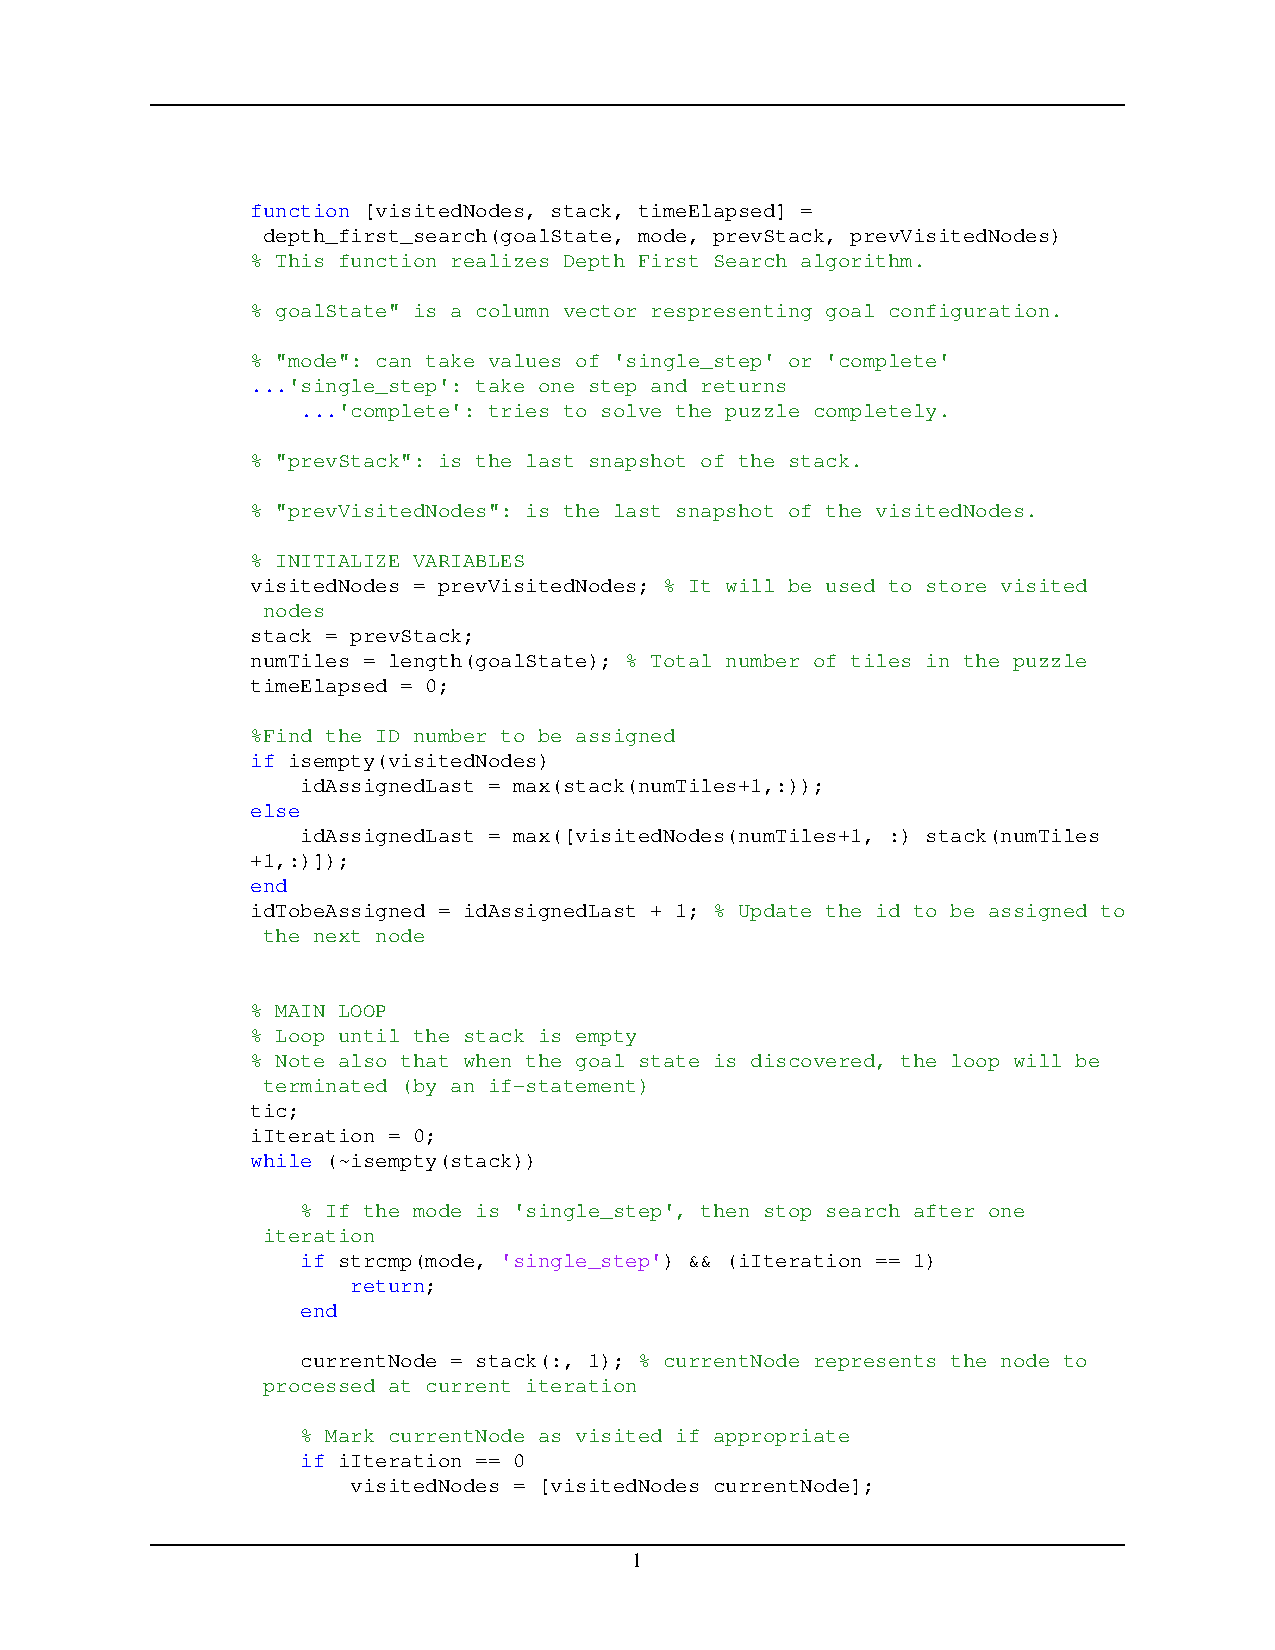
\includegraphics[width=1\columnwidth]{images/Code_depth_first_search.pdf}
	\caption{Implementation: \textit{depth\_first\_search} function}
	\label{}
\end{figure}

\begin{figure}[htb]
	\centering
	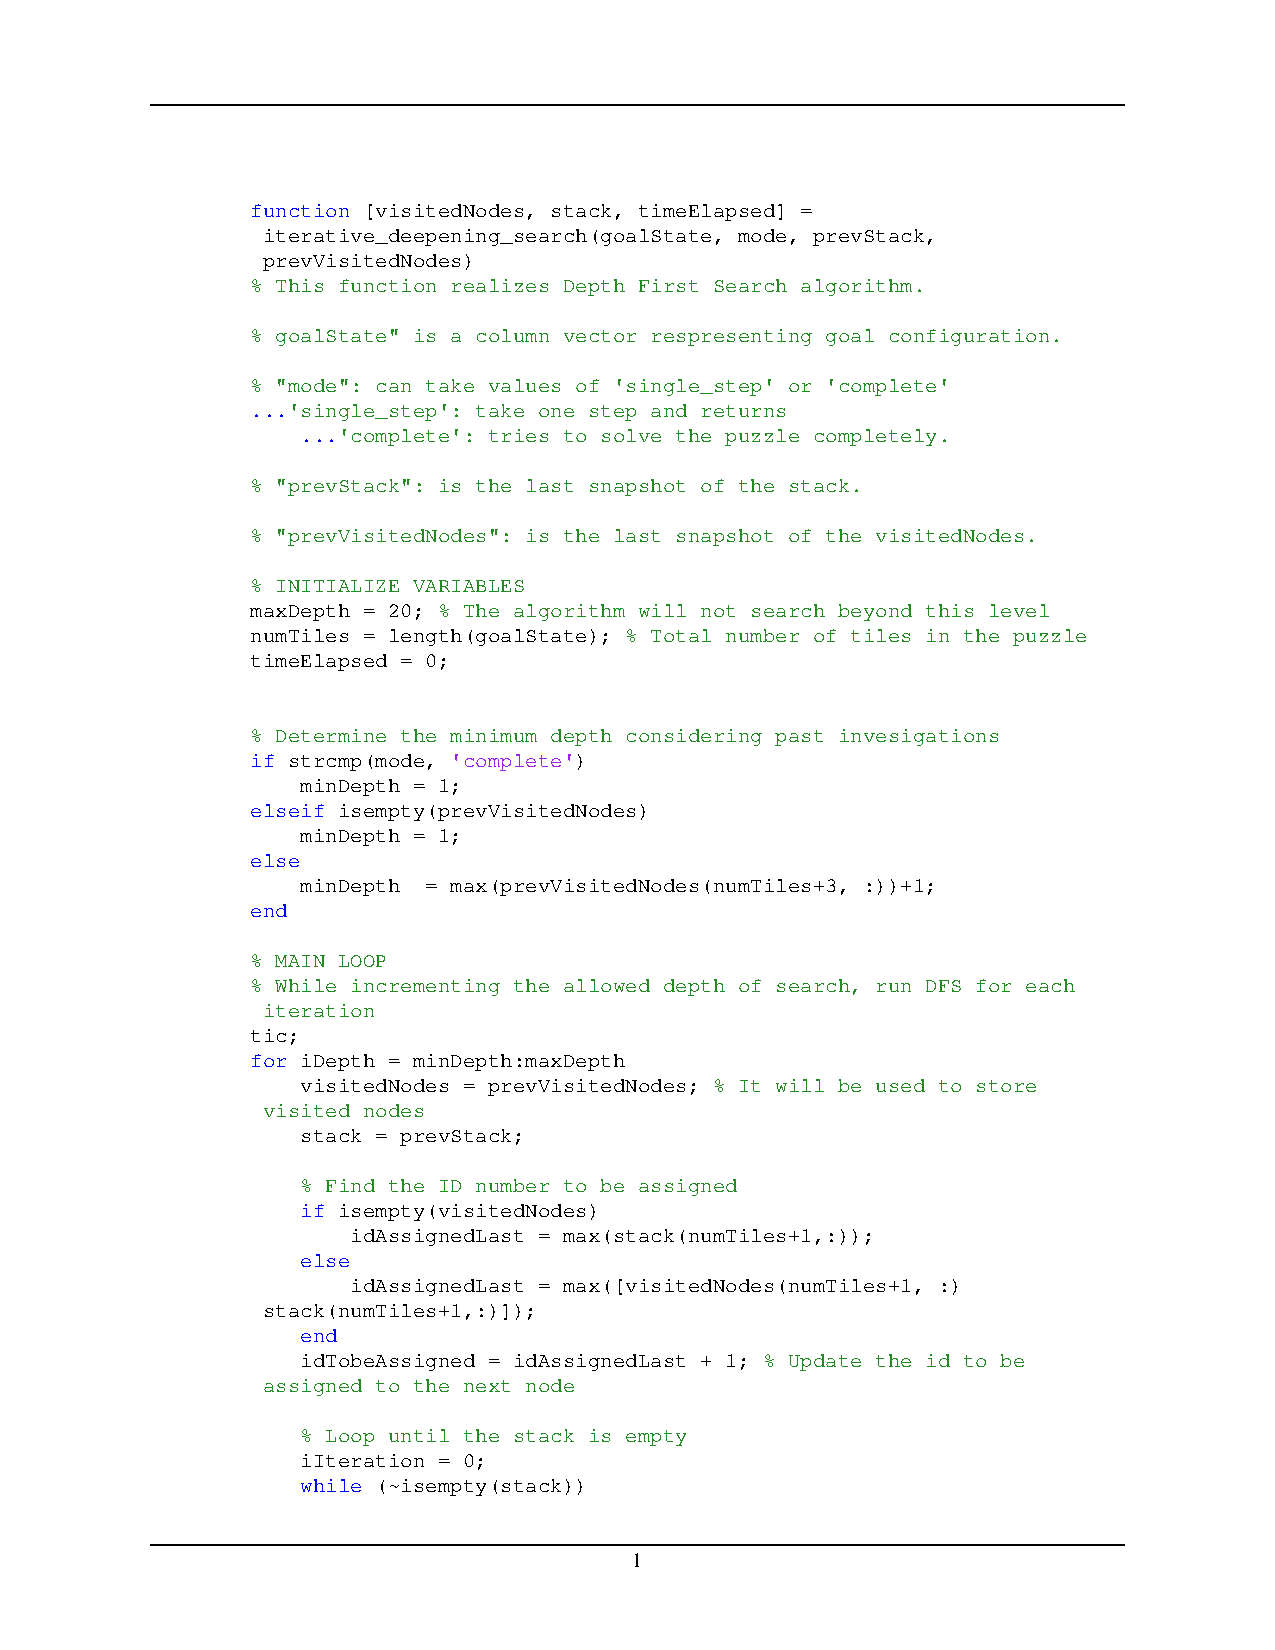
\includegraphics[width=1\columnwidth]{images/Code_iterative_deepening_search.pdf}
	\caption{Implementation: \textit{iterative\_deepening\_search} function}
	\label{}
\end{figure}

\begin{figure}[htb]
	\centering
	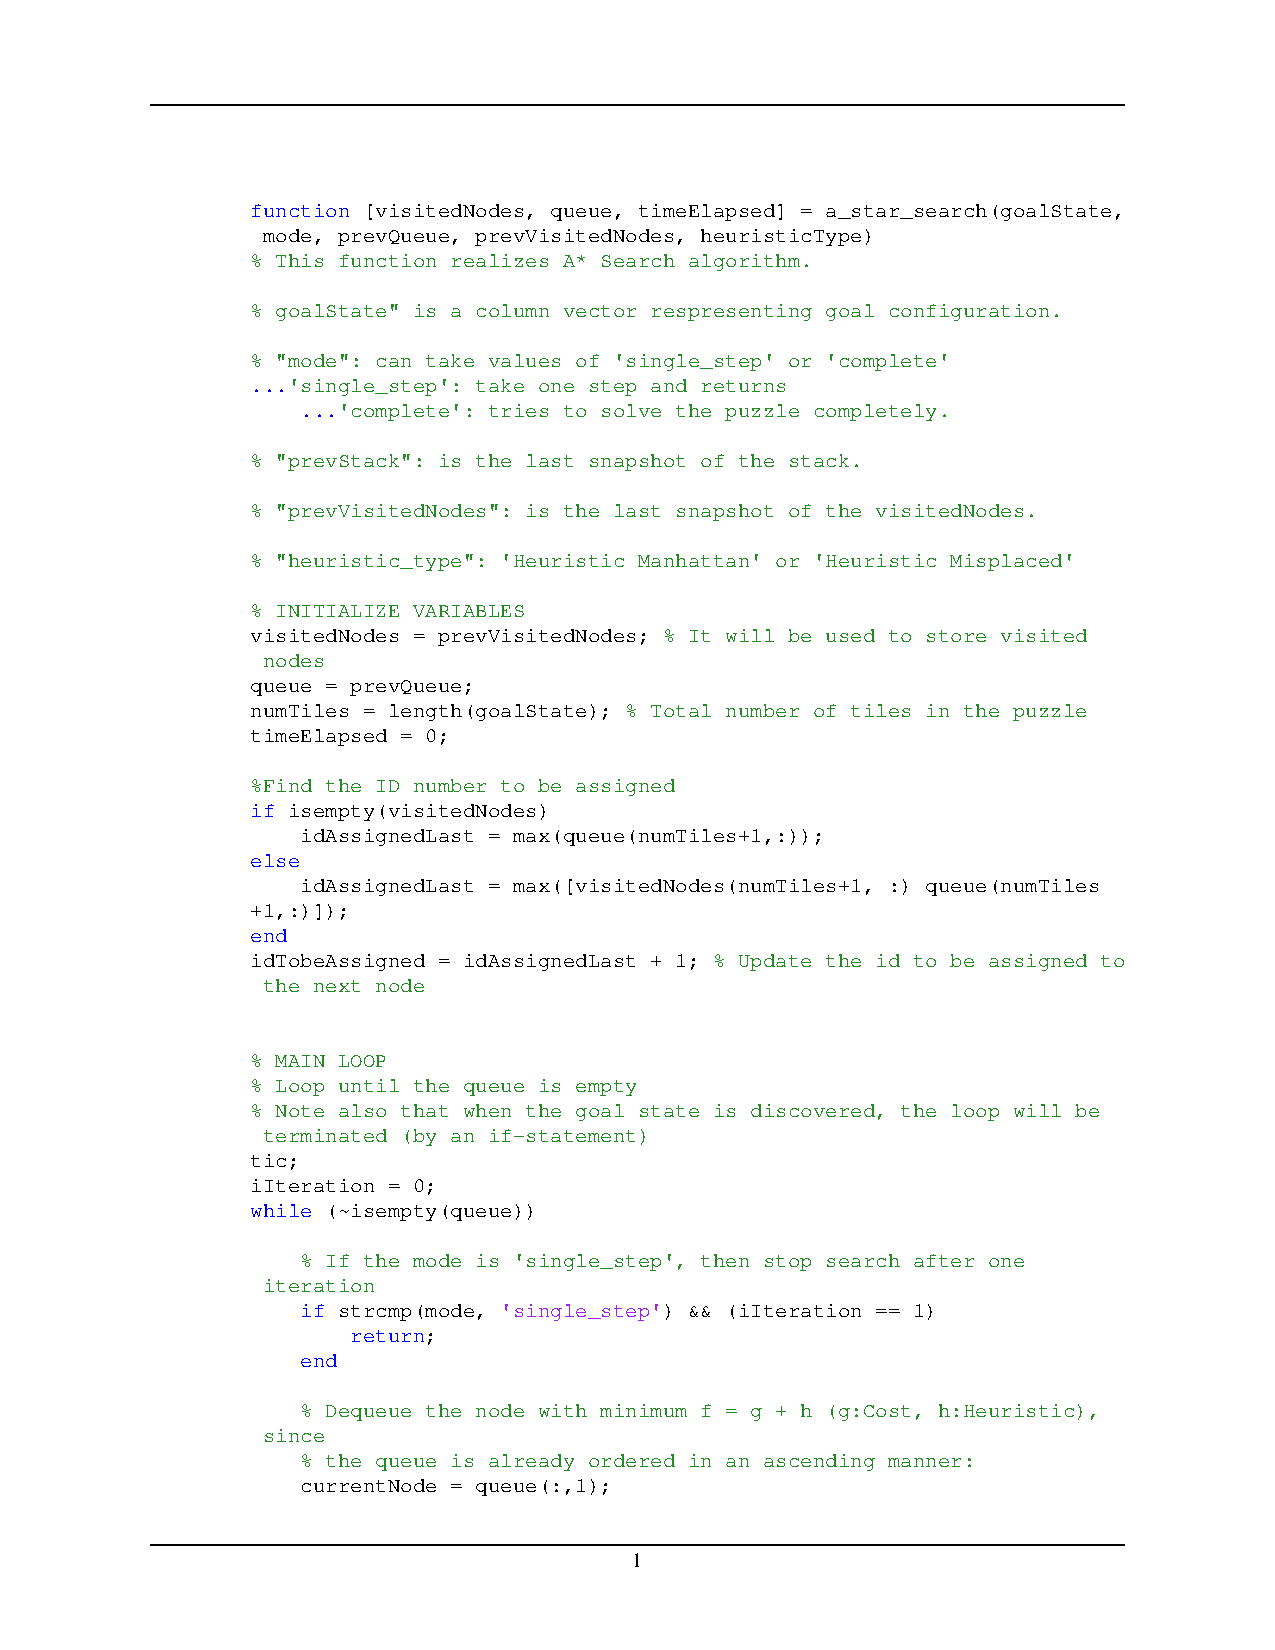
\includegraphics[width=1\columnwidth]{images/Code_a_star_search.pdf}
	\caption{Implementation: \textit{a\_star\_search} function}
	\label{}
\end{figure}

\begin{figure}[htb]
	\centering
	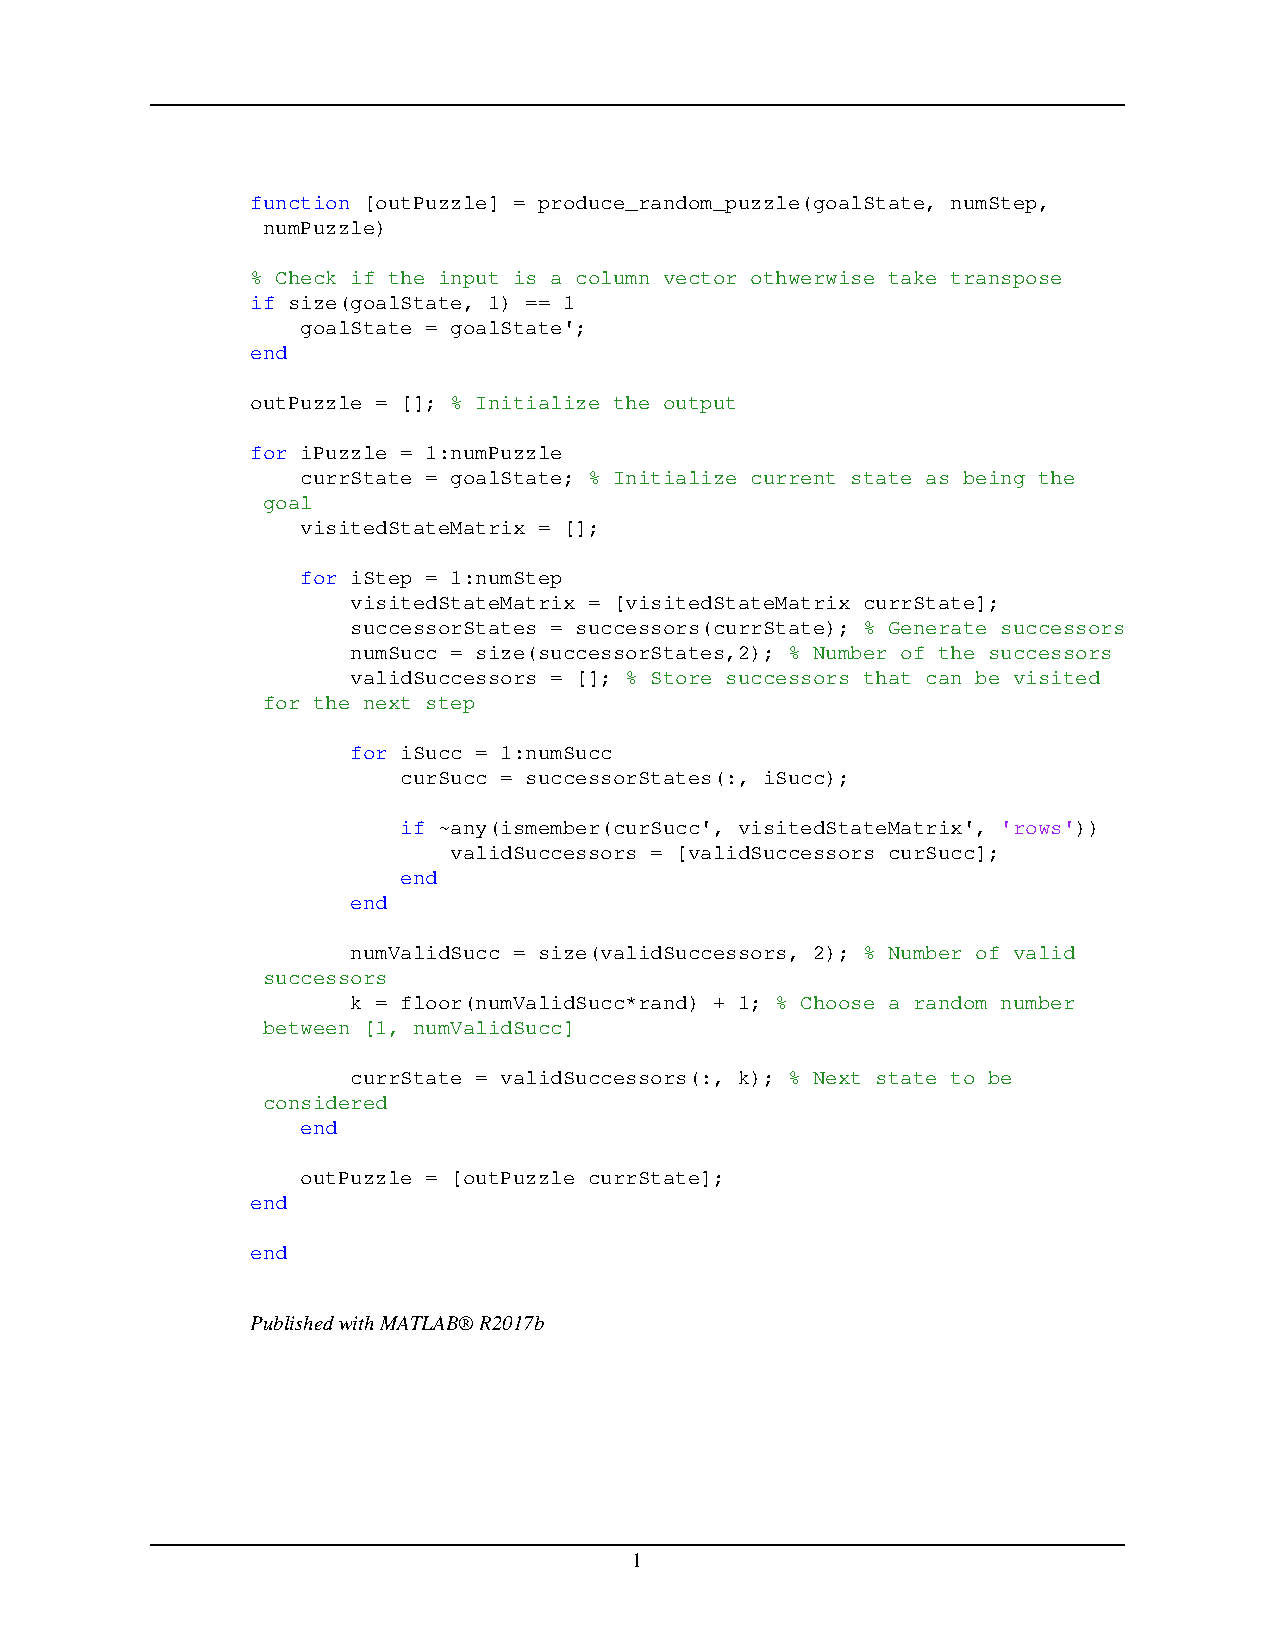
\includegraphics[width=1\columnwidth]{images/Code_produce_random_puzzle.pdf}
	\caption{Implementation: \textit{produce\_random\_puzzle} function}
	\label{}
\end{figure}

%%%%%%%%%%%%%%%%%%%%%%%%%%%%%%%%%%%%%%%%%%%%%%%%%%%%%%%%%%%%%%%%%%%%%%%%%%%%%%%%%%%%%%%%%%
%\newpage
%\bibliographystyle{plain}
%\bibliography{biblist}

\end{document}